\documentclass[conference]{IEEEtran}
\IEEEoverridecommandlockouts


\newcommand{\CC}[1]{\textcolor{blue}{#1}}

\usepackage{cite}
\usepackage{amsmath,amssymb,amsfonts}
\usepackage{graphicx}
\usepackage{textcomp}
\usepackage{xcolor}
\usepackage{booktabs}
\usepackage{array}
\usepackage{url}
\usepackage{float}
\usepackage{multirow}

\raggedbottom
\setlength{\emergencystretch}{1.5em}
\newcolumntype{L}[1]{>{\raggedright\arraybackslash}p{#1}}

\def\BibTeX{{\rm B\kern-.05em{\sc i\kern-.025em b}\kern-.08em
    T\kern-.1667em\lower.7ex\hbox{E}\kern-.125emX}}

\makeatletter
\def\ps@IEEEtitlepagestyle{%
    \def\@oddfoot{\mycopyrightnotice}%
    \def\@evenfoot{}%
}
\def\mycopyrightnotice{%
    {\raggedright \footnotesize XXX-X-XXXX-XXXX-X/26/\$XX.XX \copyright 2026 IEEE\hfill}
}
\makeatother

\begin{document}

\title{\CC{Quest Align: Real-Time Trunk Posture Awareness Using Sparse VR Tracking and Smartphone IMU Sensing}}

\author{
\IEEEauthorblockN{Carlos Castro}
\IEEEauthorblockA{\textit{School of Mathematical and Computational Sciences}\\
\textit{Yachay Tech University}\\
Urcuqu\'i, Ecuador\\
carlos.castro@yachaytech.edu.ec}
\and
\IEEEauthorblockN{Manuel Mu\~noz}
\IEEEauthorblockA{\textit{School of Mathematical and Computational Sciences}\\
\textit{Yachay Tech University}\\
Urcuqu\'i, Ecuador\\
manuel.munoz@yachaytech.edu.ec}
}

\maketitle

\begin{abstract}
\CC{This paper presents Quest Align, a real-time trunk-posture-awareness prototype that
combines sparse virtual-reality tracking with smartphone inertial sensing for
posture-oriented feedback. The system uses a pretrained HMD-Poser reconstruction backbone
and contributes the runtime and interpretation layer that connects heterogeneous consumer
sensors to the resulting SMPL pose. The framework (i)~acquires and time-synchronizes head-mounted-display,
controller, and smartphone IMU streams, with the phone mounted near the pelvis; (ii)~constructs
a 135-dimensional feature vector that exactly matches the official HMD-Poser pre-processing
layout, with foot channels and (when the phone is unavailable) pelvis channels explicitly
zeroed rather than padded generically; (iii)~feeds the model a genuine 40-frame temporal
window and recovers trunk orientation through full forward kinematics over the 22-joint
SMPL hierarchy, converted into interpretable pitch and lateral-roll indicators; and
(iv)~applies neutral calibration, threshold-based alerts, and structured real-time session
logging. The smartphone IMU is required for the intended multimodal posture-estimation mode;
headset-only operation is retained solely as a diagnostic fallback in which pelvis channels
are zeroed rather than substituted by a synthetic gravity prior. A functional evaluation was
conducted with 10~participants performing a controlled posture protocol comprising centered,
forward-flexion, and lateral-inclination states, yielding $N=1{,}504$ observer-labeled
frame-level samples (excluding calibration frames) recorded at an unweighted mean
session-level synchronized-pair frequency of 5.0~Hz (range 2.7--6.7~Hz), well below the
60~Hz rate used to train the HMD-Poser checkpoint. The resulting posture classification
achieved 66.62\% accuracy, a macro-averaged F1-score of 0.6805, and Cohen's~$\kappa$ of
0.4851. These results demonstrate operational feasibility but not biomechanical validity,
because no synchronized optical motion-capture, inclinometer, or radiographic reference was
collected, and the pelvis-only sensor configuration was not among HMD-Poser's original
training configurations.}
\end{abstract}

\renewcommand\IEEEkeywordsname{Keywords}
\begin{IEEEkeywords}
\CC{virtual reality, trunk posture awareness, HMD-Poser, SMPL, inertial measurement unit,
sparse motion tracking, real-time feedback}
\end{IEEEkeywords}

% NOTE FOR COMPILATION: rename "abtract _grafico.png" to "abstract_grafico.png"
% before building the PDF.
\begin{figure*}[t]
\centering
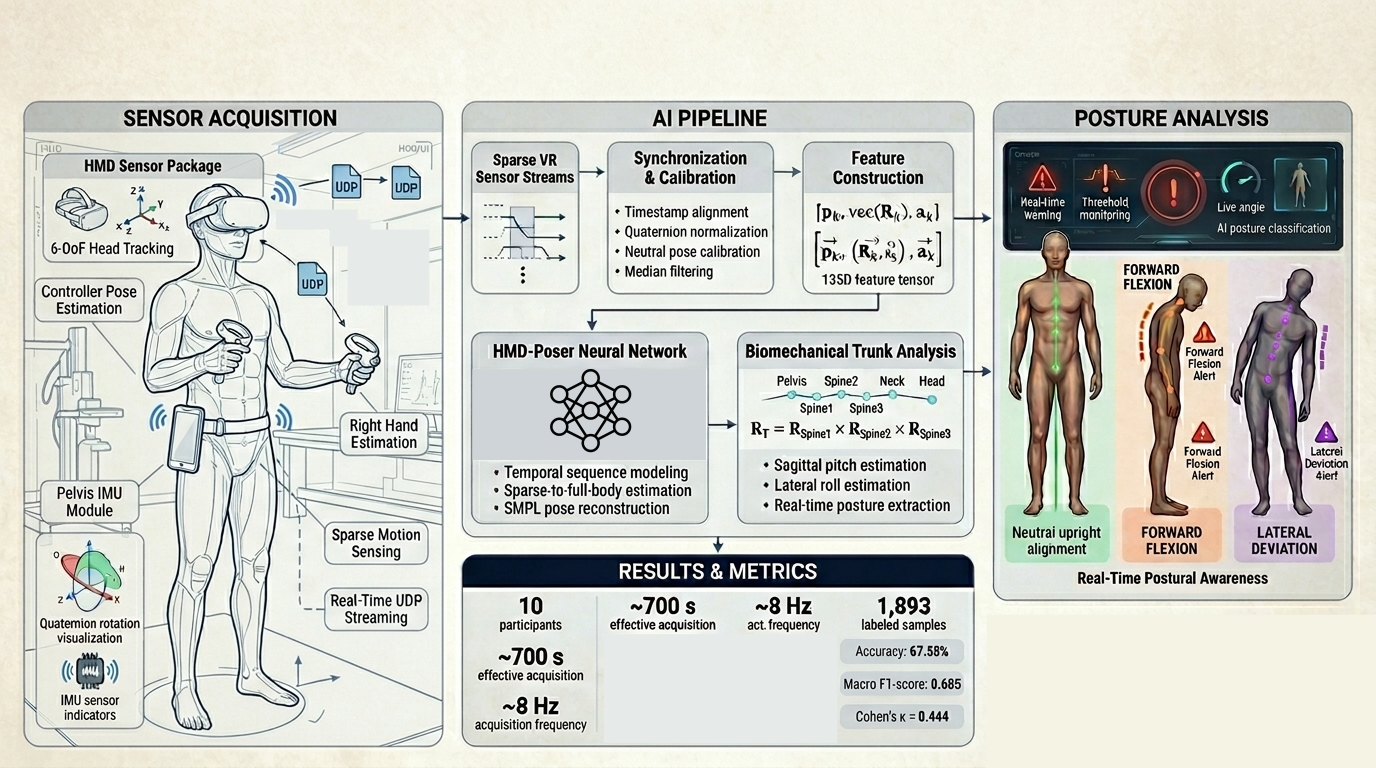
\includegraphics[width=0.82\textwidth]{abtract _grafico.png}
\caption{System overview and graphical abstract of Quest Align. The workflow is organized into four
main stages: (1)~\textit{Sensor Acquisition} via a 6-DoF VR head-mounted display with hand controllers
and a pelvis-mounted smartphone IMU streaming over UDP; (2)~\textit{AI Pipeline} encompassing
time-synchronized feature construction and the HMD-Poser backbone for sparse full-body pose
estimation; (3)~\CC{\textit{Trunk-Posture Interpretation}} providing real-time postural-awareness feedback for neutral
upright, forward-flexion, and lateral-deviation states; and (4)~\textit{Results \& Metrics}
summarizing the controlled-protocol evaluation over \CC{$N=1{,}504$} labeled frame-level samples (excluding calibration frames).}
\label{fig:system_overview}
\end{figure*}

\section{Introduction}
Musculoskeletal disorders linked to sustained poor trunk alignment rank among the most
prevalent occupational health concerns, with a substantial fraction of workers who spend
extended periods at screens or performing repetitive tasks affected over time~\cite{wearablesreview}.
Postural monitoring is therefore relevant in ergonomics, rehabilitation, human-computer
interaction, sports training, and extended computer use. Poor trunk alignment during
repetitive tasks may be difficult to notice, especially when attention is focused on a screen
or on an immersive virtual task. Conventional posture assessment can involve observation by
a specialist, manual inclinometers, marker-based motion capture, depth cameras, or
body-worn inertial measurement units~(IMUs). These tools can be useful, but many of them
require external equipment, fixed acquisition spaces, or preparation time incompatible with
ordinary VR sessions.

Modern virtual-reality~(VR) systems already include sensors that estimate the position and
orientation of the head and hands. These measurements are designed mainly for interaction
and avatar animation, but they also provide a compact description of upper-body motion.
The main limitation is that the spine, pelvis, and lower limbs are not directly observed in
a standard headset-and-controller setup. Estimating trunk posture from sparse data is
therefore an under-constrained problem: the same head-and-hand configuration may correspond
to several possible spine and pelvis configurations. Learning-based full-body reconstruction
methods address this limitation by using motion priors learned from large motion-capture
datasets~\cite{hmdposer,avatarposer,hmdnemo}.

\CC{Quest Align explores whether sparse VR body reconstruction can be repurposed for
real-time trunk-posture awareness. Instead of using a reconstructed pose only for avatar
animation, the system selects the SMPL trunk chain and derives coarse orientation-based
indicators associated with forward flexion and lateral inclination. An overview of the
end-to-end framework is depicted in
Fig.~\ref{fig:system_overview}.}

\CC{The main contribution of Quest Align is a system-level framework that repurposes sparse
full-body reconstruction from consumer VR sensors for real-time trunk-posture awareness.
The framework introduces the following components: (1)~a multimodal runtime
architecture that receives head-mounted-display, controller, and smartphone IMU
streams and synchronizes them using server-side arrival timestamps; (2)~a sensor-to-model
adaptation layer that normalizes the incoming measurements and constructs a 135-dimensional,
model-compatible feature vector following the official HMD-Poser layout; (3)~a
posture-interpretation layer that reduces the predicted SMPL trunk chain, via full forward
kinematics, into calibrated pitch and lateral-roll indicators for real-time feedback and
structured session logging; and (4)~a controlled functional evaluation with 10~participants
and 1,504 observer-labeled frame-level samples (calibration frames excluded), used to characterize acquisition consistency
and preliminary discrimination among centered, forward-flexion, and lateral-deviation
states.}

\section{Background and Related Work}
\subsection{Sparse Motion Reconstruction and Body Representation}
Sparse body tracking estimates unobserved joints from a small number of measured body
parts. In mobile VR, the usual input is the six-degree-of-freedom motion of the head and
hands. AvatarPoser showed that articulated full-body pose can be inferred from sparse
motion sensing, making full-body avatar animation possible with fewer
trackers~\cite{avatarposer}. HMD-NeMo addressed online avatar motion generation from sparse
head-mounted-display observations and emphasized latency-aware inference for interactive
scenarios~\cite{hmdnemo}. SparsePoser investigated real-time reconstruction from a reduced
tracker set and demonstrated the value of learned motion priors in sparse tracking
tasks~\cite{sparseposer}.

\CC{HMD-Poser is the closest technical basis for the present system. It recovers full-body
motion from scalable sparse observations involving an HMD and optional body-worn IMUs.
Quest Align uses its SMPL predictions as input to a sensor-adaptation and
posture-interpretation runtime comprising synchronized packet handling, feature construction,
trunk-chain selection, forward-kinematics rotation composition, neutral calibration, posture
cues, and structured session logging.}

\CC{Recent research has extended sparse full-body reconstruction toward
consumer inertial devices, dynamic motion modeling, and flexible sensor
configurations. IMUPoser and MobilePoser estimate full-body pose from inertial
sensors already available in smartphones, smartwatches, and earbuds, while
highlighting challenges related to sensor noise, drift, and temporal
consistency~\cite{imuposer,mobileposer}. DynaIP and DiffusionPoser address
dynamic reconstruction and operation with limited or variable sensor
configurations~\cite{dynaip,diffusionposer}, whereas IMUCoCo explicitly
considers changes in the number and placement of body-worn
IMUs~\cite{imucoco}. Together, these studies show that temporal history,
sensor availability, placement, and real-device noise are central aspects of
sparse motion reconstruction.}

\CC{AvatarPoser, HMD-NeMo, SparsePoser, and HMD-Poser primarily address full-body motion reconstruction or avatar control from sparse observations. Their main contribution lies in estimating unobserved body motion from limited tracking signals rather than in providing posture-specific interpretation. Quest Align builds on this research direction but addresses a different downstream problem: it converts a reconstructed SMPL trunk chain into calibrated pitch and lateral-roll indicators, posture cues, and structured session records. Therefore, these systems are not treated as direct experimental baselines for Quest Align; instead, they provide the reconstruction foundations on which its posture-oriented runtime is built.}

The body representation used by Quest Align follows the SMPL kinematic structure because
HMD-Poser predicts SMPL-compatible joint motion. SMPL is a skinned parametric body model
that represents human shape and pose in a graphics-compatible formulation~\cite{smpl}.
AMASS provides a large archive of motion-capture sequences expressed as surface shapes and
SMPL parameters~\cite{amass}, making it useful for training and evaluating full-body
reconstruction methods. The pose output uses 6D rotation representations, which are
preferred in neural settings because they avoid the discontinuities that arise with
lower-dimensional rotation encodings such as Euler angles or
quaternion-halving~\cite{zhou6d}.



\subsection{Wearable Posture Monitoring and Sensor Calibration}
Wearable posture systems have been investigated for rehabilitation support, exercise
feedback, and everyday musculoskeletal monitoring. Simpson~\textit{et al.}~reviewed
wearable technologies for spinal posture analysis and reported that live feedback and
inertial sensing are common directions in this field~\cite{wearablesreview}. Earlier
trunk-monitoring studies used inertial sensors to estimate orientation changes in the
sagittal and frontal planes~\cite{trunk_monitoring}. Other systems implement real-time
bad-posture alerts or sensor-array feedback during exercise~\cite{realtime_posture,sensor_array}.

Compared with these systems, Quest Align reduces the number of dedicated body-worn sensors.
The headset provides the main spatial reference, the controllers give upper-body context,
and the smartphone IMU supplies the inertial channel required by the intended Quest Align
posture-estimation configuration. The phone is mounted near the pelvis, although its coordinate
frame still requires calibration to be interpreted relative to the body. This design is not
anatomically as detailed as a multi-IMU spine system, but it may be more convenient for
applications where the user is already wearing a VR headset.

\CC{Prior wearable systems have already demonstrated that trunk or sitting posture can be
monitored using dedicated body-worn sensors and that real-time feedback can be delivered to
the user. Wong and Wong used three inertial sensor modules to estimate trunk posture changes
in the sagittal and coronal planes during daily activities~\cite{trunk_monitoring}. Tlili
\textit{et al.} proposed a smart belt equipped with inertial sensors, cloud processing, and
mobile applications that provide real-time sound and visual notifications when bad sitting
posture is detected~\cite{realtime_posture}. Caviedes \textit{et al.} developed a wearable
stretch-sensor array for spine-posture monitoring and exercise biofeedback rather than an
IMU-based system~\cite{sensor_array}.}

\CC{Recent posture-feedback systems also show that sensing accuracy and feedback design
must be evaluated separately. Pereira \textit{et al.} developed a wearable
smartphone-based multisensory system for torso-posture correction and evaluated it with a
within-subjects protocol~\cite{smartphone_torso_feedback}. ERG-AI analyzed long-term
occupational postures from multiple wearable accelerometers and incorporated predictive
uncertainty into the generation of worker-oriented risk explanations and
recommendations~\cite{ergai}. In a camera-based setting, OffiStretch assessed body pose in
real time and provided interactive visual guidance during stretching, while also examining
user experience and the suitability of different feedback elements~\cite{offistretch}.
Consequently, Quest Align should not be positioned as the first posture-alert system. Its
distinction is the integration of consumer VR tracking, a smartphone inertial cue
placed near the pelvis, sparse pose reconstruction, and a posture-oriented trunk
interpretation layer within the same runtime.}

\CC{Wearable motion analysis requires transforming measurements from the
sensor coordinate frame into a meaningful body-segment frame. Recent work has
addressed this problem through simulation of inertial noise and calibration
errors, dynamic on-body calibration, and explicit analysis of
sensor-to-segment misalignment~\cite{pnp,transformer_imu_calibrator,potter_alignment}.
These findings are directly relevant to a smartphone placed near the pelvis,
because changes in fixation or attachment orientation may modify the measured
quaternion without representing an equivalent anatomical pelvis rotation.
Accordingly, the neutral-pose calibration matrix used by Quest Align to map Android
orientation into the internal frame should be interpreted as a runtime baseline
correction rather than as a fully validated sensor-to-segment calibration.}

\subsection{Real-Time and Biomechanical Evaluation}

\CC{Real-time operation and biomechanical validity represent separate
evaluation requirements. System-level performance should be characterized using
the effective sensor, synchronization, inference, and valid-output rates,
together with end-to-end latency, jitter, packet loss, and reconnection
duration~\cite{mobileposer,diffusionposer,ultrainertialposer}. Biomechanical
validation additionally requires synchronized comparison with a reference
instrument. Recent IMU validation studies have assessed trunk or full-body
measurements against camera-based or optoelectronic systems using angular
error, root-mean-square error, bias, correlation, and limits of
agreement~\cite{ali_trunk_validation,camptocormia_imu,villa_imu_validation}.
Consequently, Quest Align's nominal server frequency and observer-labeled
posture classification demonstrate functional operation, but they do not
establish angular agreement or biomechanical measurement validity.}

\CC{Taken together, the recent literature identifies three distinct research questions.
First, sparse pose-reconstruction studies examine how accurately unobserved body motion can
be recovered from limited and heterogeneous sensors. Second, posture-feedback studies
examine how inferred states should be communicated and whether feedback is useful or
distracting. Third, biomechanical-validation studies examine agreement with reference
instruments and the influence of calibration, placement, and coordinate definitions. Quest
Align currently addresses the systems-integration question and provides a preliminary
posture-state evaluation, but it does not yet resolve the biomechanical-agreement or
longitudinal user-feedback questions. This separation defines both the contribution and the
current boundary of claims.}

\section{System Design}
\subsection{Design Requirements}
The prototype was designed around five practical requirements. The first is low setup
complexity: a headset, its controllers, and a smartphone should be sufficient to run a
session. The second is real-time operation, because posture feedback is only useful if the
user receives it during the activity. The third is robustness to partial sensing: if the
phone stream becomes unavailable, the system continues in a Quest-only fallback mode rather
than interrupting the session. This fallback has reduced observability because it lacks the
pelvis-proximal inertial evidence that is designed to improve posture discrimination; the
smartphone IMU therefore remains part of the full Quest Align configuration. The fourth is
reproducible logging, so that each session can be inspected after acquisition. The fifth is
explicit separation between functional monitoring and clinical diagnosis.

These requirements guided a four-stage pipeline: acquisition, synchronization, feature
construction, and posture reduction. Each stage is intentionally modular so that failure
points can be identified during laboratory testing.

\subsection{Hardware and Software Roles}
The headset-side stream provides the position and orientation of the head, the left hand,
and the right hand. \CC{The Android-side stream provides the smartphone orientation quaternion and acceleration vector measured near the pelvis. The Android sender requested TYPE\_ACCELEROMETER\_UNCALIBRATED when available and fell back to TYPE\_ACCELEROMETER; TYPE\_LINEAR\_ACCELERATION was not used. Smartphone orientation was obtained from TYPE\_ROTATION\_VECTOR and converted with SensorManager.getQuaternionFromVector, producing normalized quaternions transmitted in [w,x,y,z] order. The sender also transmitted three-axis gyroscope measurements (TYPE\_GYROSCOPE\_UNCALIBRATED with fallback to TYPE\_GYROSCOPE), although the gyroscope was not used in the current HMD-Poser feature tensor. Sensor listeners were registered with SENSOR\_DELAY\_GAME, and UDP packets were scheduled every 16 ms, corresponding to a nominal transmission target of approximately 62.5 Hz. The application advertised a nominal IMU rate of 60 Hz. Packet timestamps were generated using SystemClock.elapsedRealtimeNanos at packet construction and did not correspond directly to SensorEvent.timestamp. The Android destination address and UDP port were configured through the application interface and set to port 5005 during the reported acquisition sessions. The effective synchronized-pair rate was measured independently at the server. This additional channel is intended to reduce ambiguities that cannot be resolved from head-and-hand tracking alone; its specific contribution must be quantified in a future sensor-ablation study.} The headset stream uses UDP port 5006. \CC{The server loop has a nominal target of 60~Hz and tracks the most recent
timestamp for each stream; this configuration value is not the effective recording rate,
which is instead governed by the rate of accepted synchronized sensor pairs.}
\footnote{\url{https://github.com/carloscastro4172/Quest-Align}}

At the software level, the runtime is organized into four logical components. A UDP
reception layer isolates network input from the main loop and forwards headset and
smartphone packets to their corresponding handlers. A feature-construction layer
normalizes quaternions, converts them to rotation matrices, and assembles the
135-dimensional model-input vector following the official HMD-Poser layout, with
unavailable channels (feet, and pelvis in degraded mode) explicitly zeroed. A
posture-analysis layer reduces the predicted SMPL trunk rotations, via forward kinematics,
to pitch and lateral-roll indicators. Finally, a central orchestration layer
manages the acquisition state machine, stream synchronization, neutral calibration,
real-time alerts, and structured session storage. The key parameters governing
synchronization and alert generation are summarized in
Table~\ref{tab:runtime_params}.

\begin{table}[t]
\caption{\CC{Runtime parameters used in the Quest Align prototype (refactored pipeline)}}
\label{tab:runtime_params}
\centering
\renewcommand{\arraystretch}{1.15}
\begin{tabular}{ll}
\toprule
Parameter & Value \\
\midrule
Headset UDP port          & 5006 \\
Android UDP port          & 5005 \\
Nominal main-loop target  & 60~Hz \\
Sensor timeout            & 0.5~s \\
\CC{Synchronization tolerance} & \CC{200~ms} \\
\CC{Max.\ temporal-window gap} & \CC{200~ms} \\
\CC{Temporal window} & \CC{40~frames (genuine, non-repeated)} \\
\CC{Posture-offset calibration window} & \CC{30~frames} \\
Alert threshold           & $15^{\circ}$ for pitch or roll \\
Minimum saved session     & 10~valid frames \\
\bottomrule
\end{tabular}
\end{table}

\section{Materials and Methods}
\subsection{Acquisition and Synchronization}
Each incoming packet is JSON decoded. The headset packet contains head and hand position
and quaternion fields. The Android packet can be a control message, a clock-synchronization
request, or an IMU sample. Only IMU samples are pushed into the synchronized data buffer.
To prevent mixing of incompatible clock origins, the server uses the packet arrival time as
the synchronization reference for both streams.

\CC{A sensor is considered inactive if no packet is received within 0.5~s. Synchronized
pairs are formed when the arrival-timestamp difference between the headset and Android
streams is below a 200~ms tolerance; pairs outside this tolerance are discarded and counted
as rejected pairs. Each unique synchronized pair is added exactly once to the rolling
temporal window (deduplicated by pair timestamp). When the phone stream is unavailable, the
program can remain active in a Quest-only diagnostic mode: rather than inserting a
synthetic placeholder quaternion or a gravity-like acceleration prior, the pelvis-related
channels of the feature vector are explicitly zeroed, consistent with the zeroing strategy
used for the absent foot channels. This fallback preserves pipeline continuity and may
continue producing provisional posture cues, but the outputs are flagged as degraded and
excluded from the multimodal evaluation reported in this paper. For posture estimation, the
first 30~valid inference frames are used to compute neutral pitch and roll offsets, which
are then subtracted from subsequent readings. No temporal smoothing filter is currently
applied to the posture-angle time series; earlier prototype iterations used a seven-frame
median filter, but this stage was removed during the refactoring that introduced the
135-dimensional feature layout and is not present in the pipeline used for the evaluation
reported here.}

\subsection{Controlled Protocol}
The acquisition protocol was designed to generate repeatable postural changes while keeping
the movements simple enough for non-expert participants. The intended protocol comprised seven 5-s stages. Four sessions contained both lateral-inclination directions and the second centered-recovery event, whereas six sessions lacked one lateral direction and the CENTRO\_2 event in the recorded event log. All available labeled frames were retained for the exploratory aggregate analysis, resulting in an unbalanced number of observations across participants and posture classes.

\begin{figure}[t]
\centering
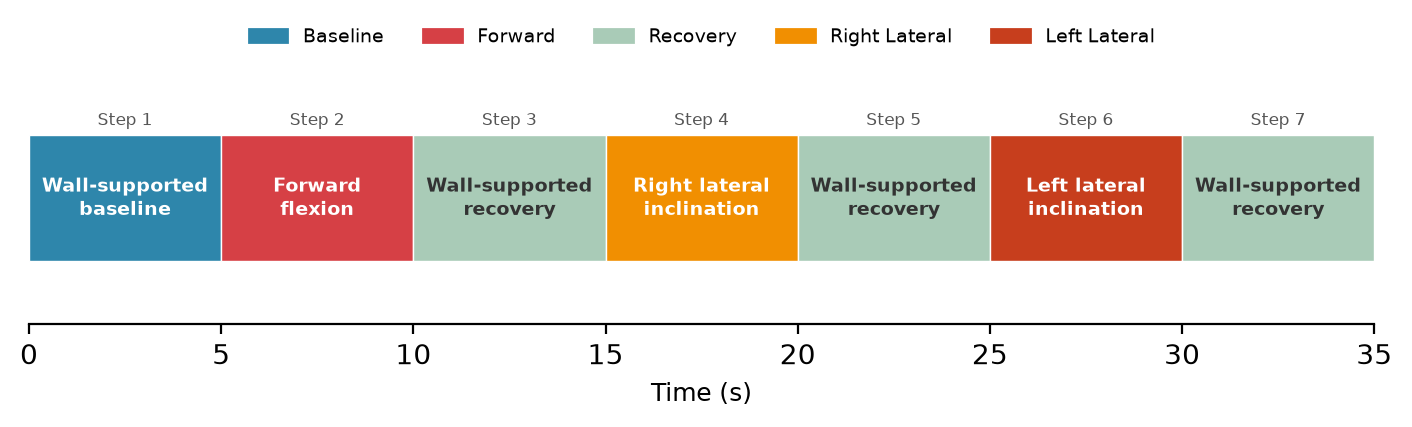
\includegraphics[width=\linewidth]{protocol_timeline.png}
\caption{\CC{Controlled posture acquisition protocol used in the evaluation (nominal timing).
The participant starts from a wall-supported upright baseline (Step~1), then performs
sequential trunk deviations: forward flexion (Step~2), right lateral inclination (Step~4),
and left lateral inclination (Step~6), each separated by 5~s wall-supported recovery
intervals (Steps~3, 5, and~7). Each step is a uniform 5~s, for a nominal total of 35~s per
participant; the mean effective session duration was 47.7~s (range 35.5--60.6~s) owing to
reconnection delays and posture-transition overhead. The server-side event log
(\texttt{step\_id} field) distinguishes six labels rather than seven, because in six of the
ten sessions one of the three wall-supported recovery segments was not logged separately
(see Table~\ref{tab:protocol_ieee}).}}
\label{fig:protocol}
\end{figure}

\begin{table}[t]
\caption{\CC{Controlled posture acquisition protocol (35~s nominal)}}
\label{tab:protocol_ieee}
\centering
\scriptsize
\renewcommand{\arraystretch}{1.18}
\resizebox{\columnwidth}{!}{%
\begin{tabular}{cllcc}
\toprule
Step & Posture condition & Reference label & Duration (s) & Cumulative time (s) \\
\midrule
1 & Wall-supported upright baseline  & Center  & 5 & 5 \\
2 & Forward trunk flexion            & Forward & 5 & 10 \\
3 & Wall-supported recovery          & Center  & 5 & 15 \\
4 & Right lateral inclination        & Lateral & 5 & 20 \\
5 & Wall-supported recovery          & Center  & 5 & 25 \\
6 & Left lateral inclination         & Lateral & 5 & 30 \\
7 & Final wall-supported recovery    & Center  & 5 & 35 \\
\midrule
\multicolumn{3}{r}{Nominal duration per participant}         & \multicolumn{2}{c}{35~s} \\
\multicolumn{3}{r}{Mean effective duration per participant} & \multicolumn{2}{c}{47.7~s (35.5--60.6~s)} \\
\multicolumn{3}{r}{Participants}                              & \multicolumn{2}{c}{10} \\
\multicolumn{3}{r}{Total effective acquisition time}          & \multicolumn{2}{c}{477.3~s} \\
\bottomrule
\end{tabular}}
\end{table}

\subsection{Participants and Ethical Considerations}
Ten adults participated in the evaluation. The sample included two participants recorded as female and eight as male. Mean age was 23.6$\pm$1.0 years (range: 22--25), mean height was 1.67$\pm$0.06 m (range: 1.56--1.75), and mean body mass was 61.7$\pm$5.4 kg (range: 53.0--69.0). Participant characteristics are reported only in aggregate to reduce re-identification risk. Participants were recruited from the university community in Ecuador. All participants provided informed consent, and the acquisition protocol was reviewed and approved by the relevant institutional ethics committee prior to data collection. The photographs in Fig.~\ref{fig:protocol} were taken and published with the participant's explicit written authorization.

\subsection{Feature Construction}
\CC{The runtime constructs a 135-dimensional feature vector per frame that exactly matches
the input pre-processing of the public HMD-Poser implementation
(\texttt{prepare\_data.py}), replacing an earlier per-sensor block layout used in initial
prototype iterations. The vector is partitioned into nine semantic blocks: (i)~global 6D
rotations for the six body segments head, left hand, right hand, left foot, right foot, and
pelvis (36 values); (ii)~global 6D rotation deltas (36 values); (iii)~global positions for
head, left hand, and right hand (9 values); (iv)~position deltas (9 values); (v)~left/right
hand rotations relative to the head (12 values); (vi)~deltas of those relative rotations
(12 values); (vii)~left/right hand positions relative to the head (6 values); (viii)~deltas
of those relative positions (6 values); and (ix)~accelerations for left foot, right foot,
and pelvis (9 values). All quaternions are normalized before conversion to rotation
matrices, and zero-norm quaternions are rejected; the 6D representation is computed as the
first two columns of the rotation matrix, as in the official HMD-Poser code. Temporal
deltas are computed from two real consecutive frames rather than being synthesized.

Because Quest Align has no foot-worn sensors, the corresponding foot channels (global
rotation, rotation delta, and acceleration) are explicitly zeroed rather than populated
with generic padding. When the smartphone stream is unavailable, the pelvis channels are
also zeroed and the server switches to the degraded \texttt{quest\_only} mode described in
Section~IV-A; no synthetic gravity vector or placeholder quaternion is substituted.

The smartphone acceleration sensor was verified from the recovered APK as TYPE\_ACCELEROMETER\_UNCALIBRATED with fallback to TYPE\_ACCELEROMETER (gravity included, m/s$^2$). After transforming the raw acceleration into the internal right-handed coordinate frame (X right, Y up, Z forward, meters, m/s$^2$) via the current phone orientation matrix and the calibration matrix R\_internal\_from\_android, the server applies an explicit gravity-compensation step under the internal Y-up convention, subtracting [0, -9.80665, 0] m/s$^2$.}

\subsection{HMD-Poser Inference}
\CC{The pretrained checkpoint \texttt{pretrained\_model\_protocol1.pt} is loaded with
\texttt{strict=True} against the \texttt{HMD\_imu\_HME\_Universe} architecture, and a smoke
test with input shape $(1,40,135)$ completes without NaN or dimensional errors. The model
receives a sliding window of 40 genuine, temporally distinct frames rather than a single
frame repeated 40 times, since deduplicated synchronized pairs are accumulated over real
time; this corrects a limitation present in earlier prototype iterations, in which the same
frame was repeated to fill the model's temporal window. At the mean session-level rate of 5.0 Hz, 40 observations would nominally span approximately 7.8 s. However, the actual temporal span of valid windows depends on the contiguous synchronized-pair sequence and must be calculated from the timestamps of each completed window. Because the effective
synchronized-pair frequency measured across the ten experimental sessions averaged 5.0~Hz
(range 2.7--6.7~Hz), compared with the 0.67~s window implied by the 60~Hz frame rate used during HMD-Poser
training, no temporal resampling is applied to correct this mismatch. In addition, the
checkpoint's training configuration only covers \texttt{HMD}, \texttt{HMD\_2IMUs} (feet),
and \texttt{HMD\_3IMUs} (feet~+~pelvis); the Quest Align sensor layout (HMD~+~hands~+~pelvis
smartphone, with feet zeroed) is not one of these original configurations. Server selects
the local 6D pose of the last predicted frame, which is passed to the forward-kinematics
stage described next. Inference results are therefore reported as network output without
claiming that the pelvis-only configuration was validated during training.}

\subsection{Trunk Angle Extraction}
\CC{The posture module recovers the global orientation of the trunk through full forward
kinematics over the 22-joint SMPL hierarchy, rather than a direct product of the three
local spine rotations used in earlier prototype iterations. Each predicted local 6D
rotation is first converted to a rotation matrix; global joint orientations are then
propagated through the kinematic tree,
\begin{equation}
\mathbf{R}^{\text{global}}_{j} = \mathbf{R}^{\text{global}}_{\mathrm{parent}(j)}\,
\mathbf{R}^{\text{local}}_{j},
\label{eq:trunk_rotation}
\end{equation}
starting from the pelvis root ($j{=}0$). Because Spine3 (joint index~9 in the SMPL+H
kinematic table) already accumulates the pelvis, Spine1, and Spine2 rotations through
Eq.~\ref{eq:trunk_rotation}, its global orientation $\mathbf{R}^{\text{global}}_{9}$ is used
directly as the composite trunk rotation $\mathbf{R}_T$, without further multiplication.
$\mathbf{R}_T$ is decomposed into Euler angles using the ZXY convention: the X-axis
component is interpreted as the sagittal-bending (pitch) indicator, and the Z-axis
component as the lateral-deviation (roll) indicator.} Fig.~\ref{fig:spine} illustrates the
selected trunk chain. The method intentionally avoids claiming vertebra-level measurements,
because SMPL spine joints are coarse animation joints rather than anatomical vertebral
landmarks.

\begin{figure}[t]
\centering
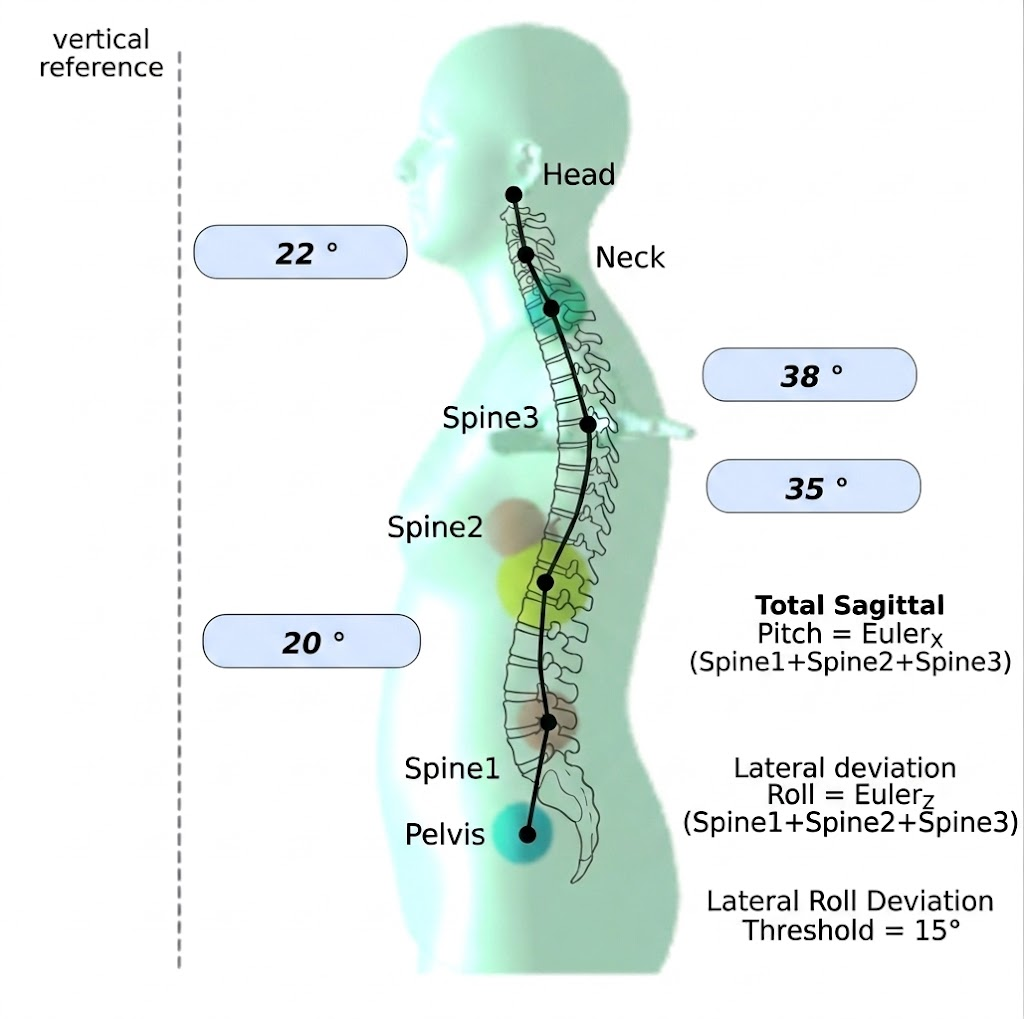
\includegraphics[width=0.95\linewidth]{spine_metrics.png}
\caption{SMPL trunk-chain joints selected for posture quantification in Quest Align. The
highlighted segment spans Pelvis through Spine1, Spine2, and Spine3. \CC{The global
orientation $\mathbf{R}^{\text{global}}_{9}$ of Spine3, obtained via forward kinematics
(Eq.~\ref{eq:trunk_rotation}), is decomposed into pitch (sagittal-bending indicator) and
roll (lateral-deviation indicator).} Vertebra-level clinical
measurements are intentionally not claimed, as these joints are coarse animation joints
rather than anatomical landmarks.}
\label{fig:spine}
\end{figure}

\subsection{Calibration and Alerts}
\CC{In the first 30~valid inference frames, the system estimates neutral pitch and roll
offsets, which are subtracted from subsequent readings; no additional smoothing filter is
applied in the pipeline used for the reported evaluation.} The alert logic is deliberately
transparent: pitch above $15^{\circ}$ indicates forward flexion, pitch below $-15^{\circ}$
indicates backward extension, and absolute roll above $15^{\circ}$ indicates lateral
deviation.

The real-time feedback is a posture-awareness cue. For example, a repeated lateral-roll
warning may indicate that the user is leaning to one side during a VR activity.

\section{Prototype Evaluation}
\subsection{Functional Verification}
The evaluation at this stage tested whether the pipeline worked end to end. The verification
covered packet parsing, sensor-state transitions, synchronization-window behavior,
quaternion normalization, feature-vector construction, loading of the pretrained model,
inference on the constructed tensor, forward-kinematics angle extraction, calibration, alert
assignment, and JSON output generation. These tests ensured that the software could receive
live signals, convert them to the model format, and produce posture feedback without manual
intervention during a recording session.

The notebook was also used to test isolated mathematical components before full integration.
Simulated trunk configurations verified that neutral and tilted postures produce consistent
changes in the expected angular channels. This component-level check reduces the risk that
runtime alerts are caused by sign errors, quaternion-format
mismatches, or incorrect joint selection.

\subsection{Outputs and Data Products}
Each session produces a structured output that can be reviewed after acquisition.
Table~\ref{tab:outputs} summarizes the data products. The key output is the per-frame
inference log containing the time series of pitch and lateral roll. Summary fields support
quick reports, while raw sensor values enable debugging when alerts are unexpected.

\begin{table}[t]
\caption{Outputs generated by Quest Align per session}
\label{tab:outputs}
\centering
\renewcommand{\arraystretch}{1.15}
\begin{tabular}{p{0.36\linewidth}p{0.53\linewidth}}
\toprule
Output & Content \\
\midrule
Sensor log        & Headset, hand, and smartphone IMU measurements with timestamps. \\
Inference log     & Pitch and roll estimates for valid frames. \\
Session summary   & Mean, minimum, and maximum posture values. \\
Calibration data  & Neutral offsets computed from early frames. \\
Alert flags       & Boolean states for forward, backward, and lateral deviations. \\
System metadata & Frame timestamps, effective rate, synchronization statistics,
configuration, calibration, and operating mode. \\
\bottomrule
\end{tabular}
\end{table}

\subsection{Controlled Posture-Orientation Test}
\CC{A controlled evaluation was conducted with 10~participants to verify whether the
refactored pipeline could distinguish three coarse posture states: Center, Lateral, and
Forward. All participants followed the nominal seven-stage protocol in Fig.~\ref{fig:protocol} and
Table~\ref{tab:protocol_ieee}, with partial event logs in six of the ten sessions. The nominal duration was 35~s per participant; the mean
effective duration was 47.7~s (range 35.5--60.6~s) owing to short reconnection losses,
posture transitions, and occasional synchronization instability. The complete acquisition
represented 477.3~s of labeled posture-monitoring data across the ten sessions, yielding
1{,}504~individually timestamped frames (calibration frames excluded).}

\CC{\textit{Runtime frequency.} The server execution loop runs at a nominal rate of
60~Hz. However, the effective end-to-end recording rate is limited by the rate of accepted
synchronized sensor pairs and is calculated from the stored frame timestamps as}
\begin{equation}
\CC{f_{\mathrm{record}}=\frac{N-1}{t_N-t_1}.}
\end{equation}
\CC{Across the ten sessions, the unweighted mean of the session-level synchronized-pair rates was 5.0 Hz, with session-level values of 6.3, 6.7, 6.2, 6.2, 4.4, 3.9, 2.7, 3.9, 6.7, and 2.7 Hz. Therefore, the nominal 60 Hz server-loop frequency should not be interpreted as the effective sensor-acquisition, synchronization, inference, or valid-output rate. An earlier 18-session dataset, collected with the initial prototype pipeline and reporting a mean rate of 7.5 Hz, is superseded by this ten-participant dataset and is not used in the analysis below.}

\CC{Each session recorded between 120 and 408 frames (mean 245), following a six-step
event log (\texttt{CALIBRACION}, \texttt{CENTRO\_1}, \texttt{INCLINACION\_ADELANTE},
\texttt{LATERAL\_DER}, \texttt{CENTRO\_2}, \texttt{LATERAL\_IZQ}) that maps onto the
nominal seven-stage protocol of Table~\ref{tab:protocol_ieee}, with the three wall-supported
recovery segments (Steps~3, 5, and~7) collapsing into at most two distinct \texttt{Centro}
labels per session; six of the ten sessions omit \texttt{CENTRO\_2} and one of the two
lateral-inclination directions. As a result, the per-class sample counts reported below are
not balanced across sessions, and this imbalance should be considered when interpreting
per-class precision and recall. Ground-truth labels were assigned by the session operator
at acquisition time; predicted labels were produced by the deployed pipeline described in
Sections~IV-D through IV-F. All 1,504~frames come from the synchronized HMD/controller-plus-smartphone
configuration; \texttt{quest\_only} diagnostic outputs were excluded from this analysis.}

Calibration frames (step\_id = CALIBRACION) were excluded from all classification metrics reported in this section because they participate in the system's neutral-offset estimation and do not constitute independent test data. The full 2,454-frame dataset including calibration frames is available in the companion repository.

\begin{figure}[H]
    \centering
    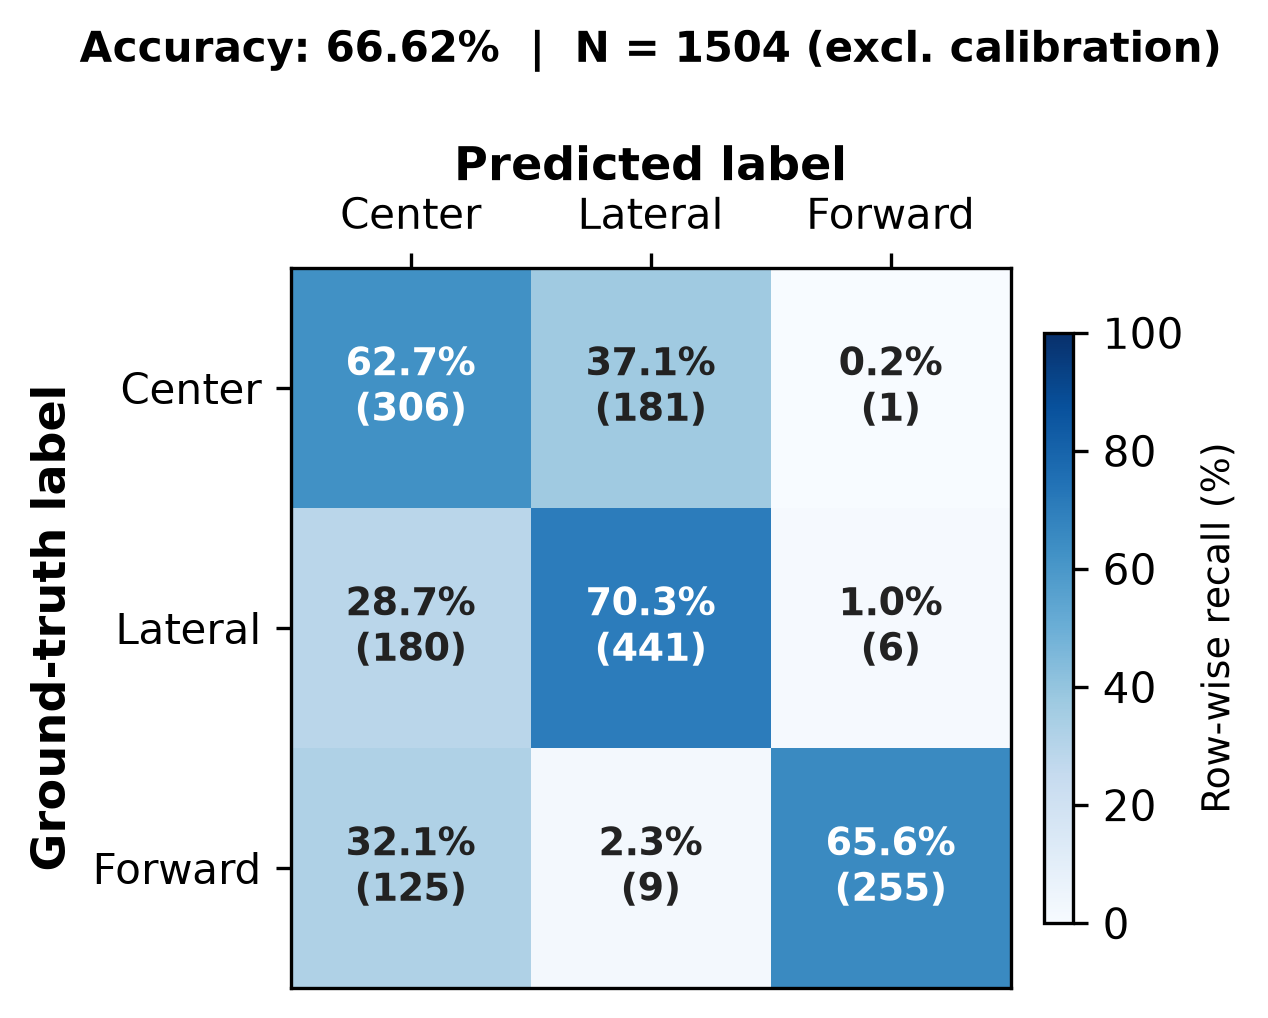
\includegraphics[width=0.90\linewidth]{confusion_matrix.png}
    \caption{\CC{Confusion matrix comparing observer-labeled posture states with Quest
    Align predictions over $N=1{,}504$ frame-level samples from the ten-participant,
    refactored-pipeline dataset. Rows represent ground-truth labels (Center, Lateral,
    Forward) and columns represent predicted labels; percentage values indicate row-wise
    recall fractions and parenthesized values indicate absolute frame counts.}}
    \label{fig:confusion_matrix}
\end{figure}

\CC{The confusion matrix in Fig.~\ref{fig:confusion_matrix} shows an overall accuracy of
66.62\%, with 1{,}002 correctly classified frames out of 1{,}504 samples (calibration frames excluded). The Center class
produced 306 true positives, 305 false positives, 711 true negatives, and 182 false
negatives. The Lateral class produced 441 true positives, 190 false positives,
687 true negatives, and 186 false negatives. The Forward class produced 255 true
positives, 7 false positives, 1{,}108 true negatives, and 134 false negatives. The main
error pattern is between Center and Lateral: 181 true Center frames were predicted as
Lateral, and 180 true Lateral frames were predicted as Center. In addition, 125 true
Forward frames were predicted as Center, suggesting that
forward-flexion events were more often confused with a return to center than with lateral
deviation.}

\begin{table}[t]
\caption{\CC{One-vs-rest counts and classification metrics for the controlled posture-orientation test ($N=1{,}504$)}}
\label{tab:posture_metrics}
\centering
\scriptsize
\renewcommand{\arraystretch}{1.15}
\resizebox{\columnwidth}{!}{%
\begin{tabular}{lrrrrrrrr}
\toprule
Class & TP & FP & TN & FN & Precision & Recall & F1-score & Specificity \\
\midrule
Center & 306 & 305 & 711 & 182 & 50.1\% & 62.7\% & 0.5569 & 70.0\% \\
Lateral & 441 & 190 & 687 & 186 & 69.9\% & 70.3\% & 0.7011 & 78.3\% \\
Forward & 255 & 7 & 1108 & 134 & 97.3\% & 65.6\% & 0.7834 & 99.4\% \\
\midrule
Macro avg. & -- & -- & -- & -- & 72.4\% & 66.2\% & 0.6805 & 82.6\% \\
\bottomrule
\end{tabular}}
\end{table}

\CC{The metric summary in Table~\ref{tab:posture_metrics} indicates that the Forward class achieves the highest precision (97.3\%) and specificity (99.4\%), but a lower recall (65.6\%), meaning that some forward-flexion frames are not detected. The Lateral class achieves the highest recall (70.3\%) with improved precision (69.9\%) after calibration-frame exclusion. The Center class shows the weakest performance, with 50.1\% precision, 62.7\% recall, and an F1-score of 0.5569. At the aggregate level, the macro-averaged F1-score is 0.6805 and Cohen's~$\kappa$ is 0.4851, indicating moderate agreement between observer labels and Quest Align predictions. The aggregate metrics are of a similar magnitude to those obtained in the earlier prototype evaluation. However, because the datasets, protocol completeness, preprocessing pipeline, and temporal representation differ, the two evaluations should not be interpreted as a controlled comparison. The remaining error is more likely attributable to the low effective sensor frequency, the pelvis-only sensor configuration (untested during HMD-Poser training), and sensor-to-segment calibration of the pelvis-mounted smartphone.}

\CC{Because consecutive frame-level samples arise from repeated measurements within the
same participants and sessions, and because the six wall-supported recovery segments are
unevenly represented across sessions (Section~V-C), these classification metrics should not
be interpreted as 1,504 statistically independent, balanced observations. Moreover,
accuracy, F1-score, and Cohen's~$\kappa$ describe agreement with observer-assigned posture
states; they do not replace angular error or agreement analysis against synchronized
biomechanical ground truth~\cite{ali_trunk_validation,villa_imu_validation}.}

\subsection{Expected Feasibility and Boundary of Claims}
The underlying real-time feasibility is supported by prior HMD-Poser experiments, but the 
present prototype does not inherit all validation results from that paper. HMD-Poser
validates full-body motion reconstruction under its own experimental protocol~\cite{hmdposer};
Quest Align adds a new downstream interpretation layer for posture feedback. That layer
must be validated separately because errors in trunk-angle estimation can arise from sensor
placement, model adaptation, calibration, and anatomical simplification.

The present result should therefore be interpreted as an observer-labeled
functional evaluation. The system can acquire, infer, extract trunk angles via forward
kinematics, alert, and store measurements, and the controlled posture protocol provides an
estimate of frame-level classification behavior on the corrected pipeline. However, these
metrics should not yet be interpreted as clinical sensitivity, clinical specificity, or
diagnostic agreement. A stronger quantitative study would require synchronized reference
data, standardized sensor placement, higher and more consistent effective sensor
frequency, and comparisons to accepted measurement instruments.

\section{Discussion}
Quest Align demonstrates that a VR headset can provide the primary spatial reference in a
posture-monitoring pipeline, while the smartphone IMU supplies the required inertial channel
for the intended multimodal configuration. The approach does not require external cameras
and can operate inside the same interaction loop as a VR application. Using a smartphone
near the pelvis avoids specialized wearable hardware, making the prototype suitable for
educational demonstrations, early ergonomic feedback studies, and laboratory investigation
of \CC{HMD-based trunk-motion analysis}.

\CC{The ten-session evaluation yielded session-level synchronized-pair rates of 6.3, 6.7, 6.2, 6.2, 4.4, 3.9, 2.7, 3.9, 6.7, and 2.7 Hz (unweighted mean 5.0 Hz), substantially below the nominal 60 Hz server-loop target.
Because the model now receives a genuine 40-frame window rather than a repeated frame, this low frequency
translates directly into a temporal-horizon mismatch: at the mean session-level rate of 5.0 Hz, 40 observations would nominally span approximately 7.8 s of real
time versus the 0.67~s window used during HMD-Poser training, and no resampling is applied
to reconcile the two. However, the actual temporal span of valid windows depends on the contiguous synchronized-pair sequence and must be calculated from the timestamps of each completed window. A future runtime benchmark should separately report sensor,
synchronization, inference, and valid-output rates together with latency, jitter, frame
loss, and reconnection intervals~\cite{mobileposer,diffusionposer,ultrainertialposer}, and
should evaluate whether temporal resampling (e.g., SLERP for orientations, linear
interpolation for positions and accelerations) narrows this mismatch and improves
classification agreement.}

The most significant limitation is \textit{anatomical resolution}. SMPL was not designed
as a clinical spine model and includes only a few joints in the trunk chain. As a result,
Quest Align estimates coarse trunk orientation rather than vertebral alignment. A system
intended for clinical use would require a more detailed body model with validated
anatomical landmarks and ground-truth comparison against radiographic or optical
motion-capture references.

\CC{Accordingly, the absence of synchronized reference measurements is not resolved by the
observer-labeled classification results. Concurrent validation should report pitch and roll
errors separately and include participant-level measures of error, bias, and agreement, as
demonstrated in recent IMU validation studies~\cite{ali_trunk_validation,camptocormia_imu,villa_imu_validation}.}

\CC{The second limitation is \textit{temporal horizon mismatch}. The single-frame-repeat
strategy used in earlier prototype iterations has been replaced with a genuine 40-frame
rolling window, which corrects the most severe form of pipeline disconnection from
HMD-Poser's temporal modeling assumptions. However, because the effective synchronized-pair
frequency (5.0~Hz on average) remains far below the checkpoint's training frequency
(60~Hz), the window still does not represent the same real-world motion horizon the network
was trained on. Recent dynamic and configuration-flexible reconstruction methods reinforce
the need to evaluate difficult motions, real sensor noise, and temporal consistency using
resampled input sequences and sensor-configuration ablations~\cite{dynaip,diffusionposer}.}

The third limitation is \textit{sensor placement}. Pocket orientation and attachment
rotation can change the phone coordinate frame and propagate bias through the pipeline.
The neutral-pose calibration matrix provides a runtime baseline, while future experiments should use
standardized attachment, controlled placement perturbations, and dynamic
recalibration~\cite{transformer_imu_calibrator,potter_alignment,imucoco}.

The fourth limitation is \textit{threshold generality}. The selected $15^{\circ}$ alert
threshold is useful for prototyping, but it should not be treated as a universal
threshold. Different tasks, users, and body proportions may require individualized
thresholds. A future calibration stage could ask the user to perform reference postures and
adapt thresholds to individual baseline kinematics, improving both specificity and user
experience.

\CC{Alert effectiveness must also be evaluated independently of posture-state
classification. Studies of multisensory, occupational, and visual posture feedback show the
importance of uncertainty, usability, distraction, and feedback modality; future Quest
Align studies should therefore compare alert formats and assess user response over longer
sessions~\cite{smartphone_torso_feedback,ergai,offistretch}.}

\section{Future Work}
\CC{The next version should address the temporal-horizon mismatch identified in Section~VI,
either by increasing the effective synchronized-pair frequency (e.g., via more efficient UDP
handling or reduced synchronization tolerance) or by implementing temporal resampling
(SLERP for orientations, linear interpolation for positions and accelerations) so that the
40-frame window more closely matches the 0.67~s horizon used during HMD-Poser training.}
A second priority is collecting a validation dataset in which each participant
performs predefined postures while the VR system records headset/controller data, the
smartphone records \CC{inertial data from a standardized location near the pelvis}, and a reference system records ground truth. Suitable
reference systems include optical motion capture, validated multi-IMU setups, or calibrated
inclinometers. The comparison should report angular error, latency, dropped-frame rate, and
robustness to phone placement.

User-facing feedback also requires dedicated study. Alerts that are too frequent may
distract users inside VR, while alerts that are too rare may fail to produce corrective
behavior. Future experiments should compare continuous numeric feedback, simple warning
icons, auditory cues, and end-of-session summaries. Privacy should also be addressed,
because motion traces can contain identifiable behavioral patterns; local on-device
processing and minimal storage are preferable when the goal is personal posture feedback.

Table~\ref{tab:validation_plan} summarizes a structured validation plan for converting the
current prototype into a quantitatively evaluated system. The plan separates technical,
biomechanical-agreement, and user-facing tests because each one addresses a distinct
research question: a system can be fast and stable but still anatomically inaccurate, and
a system can be accurate in a laboratory but distracting during an immersive task.

\begin{table}[t]
\caption{Proposed validation protocol for future quantitative evaluation}
\label{tab:validation_plan}
\centering
\renewcommand{\arraystretch}{1.15}
\begin{tabular}{p{0.30\linewidth}p{0.58\linewidth}}
\toprule
Validation aspect & Suggested measurement \\
\midrule
Synchronization   & Time offset between headset and phone samples during repeated
  movements. \\
\CC{Effective frequency} & \CC{Synchronized-pair rate and window-fill latency under
  reduced synchronization tolerance and/or temporal resampling.} \\
Angular agreement & Mean absolute error against optical motion capture, validated
  IMUs, or calibrated inclinometers. \\
Dynamic stability & Jitter and dropped-frame rate during walking, leaning, and seated
  tasks. \\
Sensor placement  & Error change when the phone is placed at different pelvis or waist
  locations. \\
User feedback     & Comfort, distraction, and perceived usefulness of alerts during
  VR tasks. \\
\bottomrule
\end{tabular}
\end{table}

\section{Conclusion}
\CC{This paper presented Quest Align, a real-time prototype that links consumer VR headset
tracking, Android inertial sensing near the pelvis, HMD-Poser sparse inference over a
genuine 40-frame temporal window, and forward-kinematics-based SMPL trunk-angle extraction
into an end-to-end posture-monitoring pipeline. The system receives UDP sensor streams,
constructs a 135-dimensional feature vector matching the official HMD-Poser layout,
estimates pitch and lateral roll, applies neutral calibration, and stores structured session
records. A controlled acquisition protocol with 10~participants (35~s nominal, 47.7~s mean
effective duration per session) produced $N=1{,}504$ observer-labeled frame-level samples (calibration frames excluded);
the classification evaluation on the refactored pipeline yielded an overall accuracy of
66.62\%, a macro-averaged F1-score of 0.6805, and a Cohen's~$\kappa$ of 0.4851, indicating
moderate agreement between observer labels and system predictions -- a result of similar
magnitude to earlier prototype iterations despite substantial corrections to the feature
layout, temporal window, and trunk-angle extraction method, suggesting that the low
effective sensor frequency and the untested pelvis-only sensor configuration are more
likely bottlenecks than the specific implementation bugs corrected during refactoring.

The work provides a reproducible implementation path for turning sparse VR tracking into
real-time postural awareness. Future validation must compare the inferred indicators
against ground-truth measurements, narrow the temporal-horizon mismatch between the
effective sensor frequency and the HMD-Poser training frequency, and standardize pelvis
sensor attachment before the system can be applied responsibly in health-related
decision-making.}


\begin{thebibliography}{26}

\bibitem{wearablesreview}
L. Simpson, M.~M. Maharaj, and R.~J. Mobbs,
``The role of wearables in spinal posture analysis: A systematic review,''
\textit{BMC Musculoskeletal Disord.}, vol.~20, no.~55, 2019,
doi: 10.1186/s12891-019-2430-6.

\bibitem{hmdposer}
P. Dai, Y. Zhang, T. Liu, Z. Fan, T. Du, Z. Su, X. Zheng, and Z. Li,
``HMD-Poser: On-device real-time human motion tracking from scalable sparse observations,''
in \textit{Proc. IEEE/CVF Conf. Computer Vision and Pattern Recognition (CVPR)},
2024, pp.~874--884,
doi: 10.1109/CVPR52733.2024.00089.

\bibitem{avatarposer}
J. Jiang, P. Streli, H. Qiu, A. Fender, L. Laich, P. Snape, and C. Holz,
``AvatarPoser: Articulated full-body pose tracking from sparse motion sensing,''
in \textit{Eur. Conf. Computer Vision (ECCV)}, vol.~13664, Springer, 2022, pp.~443--460,
doi: 10.1007/978-3-031-20065-6\_26.

\bibitem{hmdnemo}
S. Aliakbarian, F. Saleh, D. Collier, P. Cameron, and D. Cosker,
``HMD-NeMo: Online 3D avatar motion generation from sparse observations,''
in \textit{Proc. IEEE/CVF Int. Conf. Computer Vision (ICCV)}, 2023, pp.~9588--9597,
doi: 10.1109/ICCV51070.2023.00882.

\bibitem{sparseposer}
J.~L. Ponton, H. Yun, A. Aristidou, C. Andujar, and N. Pelechano,
``SparsePoser: Real-time full-body motion reconstruction from sparse data,''
\textit{ACM Trans. Graph.}, vol.~43, no.~1, Art.~5, 2023,
doi: 10.1145/3625264.

\bibitem{trunk_monitoring}
W.~Y. Wong and M.~S. Wong,
``Trunk posture monitoring with inertial sensors,''
\textit{Eur. Spine J.}, vol.~17, no.~5, pp.~743--753, 2008,
doi: 10.1007/s00586-008-0586-0.

\bibitem{realtime_posture}
F. Tlili, R. Haddad, R. Bouallegue, and N. Mezghani,
``A real-time posture monitoring system towards bad posture detection,''
\textit{Wireless Pers. Commun.}, vol.~120, pp.~1207--1227, 2021,
doi: 10.1007/s11277-021-08511-2.

\bibitem{sensor_array}
J.~E. Caviedes, B. Li, and V.~C. Jammula,
``Wearable sensor array design for spine posture monitoring during exercise incorporating
biofeedback,''
\textit{IEEE Trans. Biomed. Eng.}, vol.~67, no.~10, pp.~2828--2838, 2020,
doi: 10.1109/TBME.2020.2971907.

\bibitem{smpl}
M. Loper, N. Mahmood, J. Romero, G. Pons-Moll, and M.~J. Black,
``SMPL: A skinned multi-person linear model,''
\textit{ACM Trans. Graphics}, vol.~34, no.~6, pp.~1--16, 2015,
doi: 10.1145/2816795.2818013.

\bibitem{amass}
N. Mahmood, N. Ghorbani, N.~F. Troje, G. Pons-Moll, and M.~J. Black,
``AMASS: Archive of motion capture as surface shapes,''
in \textit{Proc. IEEE/CVF Int. Conf. Computer Vision (ICCV)}, 2019, pp.~5442--5451,
doi: 10.1109/ICCV.2019.00554.

\bibitem{zhou6d}
Y. Zhou, C. Barnes, J. Lu, J. Yang, and H. Li,
``On the continuity of rotation representations in neural networks,''
in \textit{Proc. IEEE/CVF Conf. Computer Vision and Pattern Recognition (CVPR)}, 2019,
pp.~5745--5753, doi: 10.1109/CVPR.2019.00589.

{\color{blue}
\bibitem{imuposer}
V. Mollyn, R. Arakawa, M. Goel, C. Harrison, and K. Ahuja,
``IMUPoser: Full-body pose estimation using IMUs in phones, watches, and earbuds,''
in \textit{Proc. CHI Conf. Human Factors Comput. Syst.}, 2023,
Art. no. 529, pp.~1--12,
doi: 10.1145/3544548.3581392.

\bibitem{mobileposer}
V. Xu, C. Gao, H. Hoffmann, and K. Ahuja,
``MobilePoser: Real-time full-body pose estimation and 3D human translation from IMUs in
mobile consumer devices,''
in \textit{Proc. 37th Annu. ACM Symp. User Interface Softw. Technol.},
2024, pp.~1--11,
doi: 10.1145/3654777.3676461.

\bibitem{dynaip}
Y. Zhang, S. Xia, L. Chu, J. Yang, Q. Wu, and L. Pei,
``Dynamic Inertial Poser (DynaIP): Part-based motion dynamics learning for enhanced human
pose estimation with sparse inertial sensors,''
in \textit{Proc. IEEE/CVF Conf. Comput. Vis. Pattern Recognit. (CVPR)},
2024, pp.~1889--1899,
doi: 10.1109/CVPR52733.2024.00185.

\bibitem{diffusionposer}
T. Van Wouwe, S. Lee, A. Falisse, S. Delp, and C. K. Liu,
``DiffusionPoser: Real-time human motion reconstruction from arbitrary sparse sensors using
autoregressive diffusion,''
in \textit{Proc. IEEE/CVF Conf. Comput. Vis. Pattern Recognit. (CVPR)},
2024, pp.~2513--2523,
doi: 10.1109/CVPR52733.2024.00243.

\bibitem{ultrainertialposer}
R. Armani, C. Qian, J. Jiang, and C. Holz,
``Ultra Inertial Poser: Scalable motion capture and tracking from sparse inertial sensors
and ultra-wideband ranging,''
in \textit{ACM SIGGRAPH 2024 Conf. Papers}, 2024,
Art. no. 51, pp.~1--11,
doi: 10.1145/3641519.3657465.

\bibitem{imucoco}
H. Zhou, R. Arakawa, Y. Agarwal, and M. Goel,
``IMUCoCo: Enabling flexible on-body IMU placement for human pose estimation and activity
recognition,''
in \textit{Proc. 38th Annu. ACM Symp. User Interface Softw. Technol.},
2025, Art. no. 91, pp.~91:1--91:16,
doi: 10.1145/3746059.3747695.

\bibitem{pnp}
X. Yi, Y. Zhou, and F. Xu,
``Physical Non-inertial Poser (PNP): Modeling non-inertial effects in sparse-inertial human
motion capture,''
in \textit{ACM SIGGRAPH 2024 Conf. Papers}, 2024, pp.~1--11,
doi: 10.1145/3641519.3657436.

\bibitem{transformer_imu_calibrator}
C. Zuo, J. Huang, X. Jiang, Y. Yao, X. Shi, R. Cao, X. Yi, F. Xu,
S. Guo, and Y. Qin,
``Transformer IMU Calibrator: Dynamic on-body IMU calibration for inertial motion capture,''
\textit{ACM Trans. Graph.}, vol.~44, no.~4, Art. no. 45,
pp.~45:1--45:14, 2025,
doi: 10.1145/3730937.

\bibitem{potter_alignment}
M. V. Potter,
``Simulating effects of sensor-to-segment alignment errors on IMU-based estimates of lower
limb joint angles during running,''
\textit{Sports Eng.}, vol.~28, Art. no. 1, 2025,
doi: 10.1007/s12283-024-00483-3.

\bibitem{smartphone_torso_feedback}
A. P. Pereira, O. J. Machado Neto, V. M. C. Elui, and M. da G. C. Pimentel,
``Wearable smartphone-based multisensory feedback system for torso posture correction:
Iterative design and within-subjects study,''
\textit{JMIR Aging}, vol.~8, Art. no. e55455, 2025,
doi: 10.2196/55455.

\bibitem{ergai}
S. Sen, V. Gonzalez, E. J. Husom, S. Tverdal, S. Tokas, and S. O. Tj{\o}svoll,
``ERG-AI: Enhancing occupational ergonomics with uncertainty-aware ML and LLM feedback,''
\textit{Appl. Intell.}, vol.~54, no.~23, pp.~12128--12155, 2024,
doi: 10.1007/s10489-024-05796-1.

\bibitem{offistretch}
J. Adolf, P. K{\'a}n, T. Feuchtner, B. Adolfov{\'a}, J. Dole{\v z}al,
and L. Lhotsk{\'a},
``OffiStretch: Camera-based real-time feedback for daily stretching exercises,''
\textit{Vis. Comput.}, vol.~41, no.~3, pp.~1555--1571, 2025,
doi: 10.1007/s00371-024-03450-y.

\bibitem{ali_trunk_validation}
F. Ali, C. A. Hogen, E. J. Miller, and K. R. Kaufman,
``Validation of pelvis and trunk range of motion as assessed using inertial measurement
units,''
\textit{Bioengineering}, vol.~11, no.~7, Art. no. 659, 2024,
doi: 10.3390/bioengineering11070659.

\bibitem{camptocormia_imu}
K. Naderi Beni, K. Knutzen, J. P. Kuhtz-Buschbeck, N. G. Margraf, and R. Rieger,
``Continuous mobile measurement of camptocormia angle using four accelerometers,''
\textit{Med. Biol. Eng. Comput.}, vol.~62, no.~12,
pp.~3637--3652, 2024,
doi: 10.1007/s11517-024-03149-1.

\bibitem{villa_imu_validation}
G. Villa, S. Cerfoglio, A. Bonfiglio, P. Capodaglio, M. Galli, and V. Cimolin,
``Validation of a commercially available IMU-based system against an optoelectronic system
for full-body motor tasks,''
\textit{Sensors}, vol.~25, no.~12, Art. no. 3736, 2025,
doi: 10.3390/s25123736.
}

\end{thebibliography}

\end{document}
